\documentclass{article}
\usepackage[preprint]{neurips_2026}
\usepackage{booktabs,graphicx,hyperref}
\title{Agent Skill Discovery at Scale: Matched Local Evidence}
\author{\texttt{deepujoy88}\And\texttt{speccy88}\And\texttt{vsimard}}
\begin{document}\maketitle
\begin{abstract}Research draft. We compare five discovery strategies on 200 exposed public SkillRet queries at four catalog sizes. Retrieval coverage and final set agreement are distinct. At 6,006 skills, hybrid retrieves 57.17\% of positive qrels at five candidates but produces 11 exact sets out of 200; BM25 produces 9. The paired difference is uncertain. Full listing exceeds the configured 8,192-token budget at 1000 and 6006 skills. Results concern a constrained 0.6B metadata selector, not task execution.\end{abstract}
\section{Question and scope}We evaluate the supplied proposal's accuracy and efficiency question while preserving its iterative-scope disclaimer. The original 80 hosted cells remain separately tracked. Historical studies use different panels and views and are not pooled.
\section{Related work}SkillRet supplies the retrieval benchmark \cite{kang2026skillret}. Skill retrieval augmentation \cite{su2026skill}, skill shadowing \cite{song2026shadowing} and dependency-aware structural retrieval \cite{liu2026graph} motivate distinct retrieval, selection and workflow questions. Their published results are not new measurements here.
\section{Method}We freeze 200 exposed queries with 98/78/24 one/two/three-positive strata and seed 42. Per-query gold-conditioned catalogs contain 10, 100, 1,000 and 6,006 skills. BM25 uses local IDF, k1=1.5, b=0.75; vector search uses pinned BGE-small CLS-normalized embeddings; hybrid uses equal RRF60. Domain vector routes with the same selector and no global fallback. Full listing exposes all metadata. Strict opaque-ID JSON selection returns zero to five IDs and offers no tools.
\section{Results}\begin{table}[t]\centering\small
\begin{tabular}{lrrr}\toprule Method & Exact/200 & Recall@5 & MRR@5\\\midrule
bm25 & 9 & 0.462 & 0.532\\
vector & 7 & 0.516 & 0.582\\
domain\_vector & 4 & 0.348 & 0.399\\
hybrid & 11 & 0.572 & 0.637\\
\bottomrule\end{tabular}\caption{Primary200-query sample at6006 skills. Sample-macro retrieval and raw exact counts.}\end{table}

\begin{figure}[t]\centering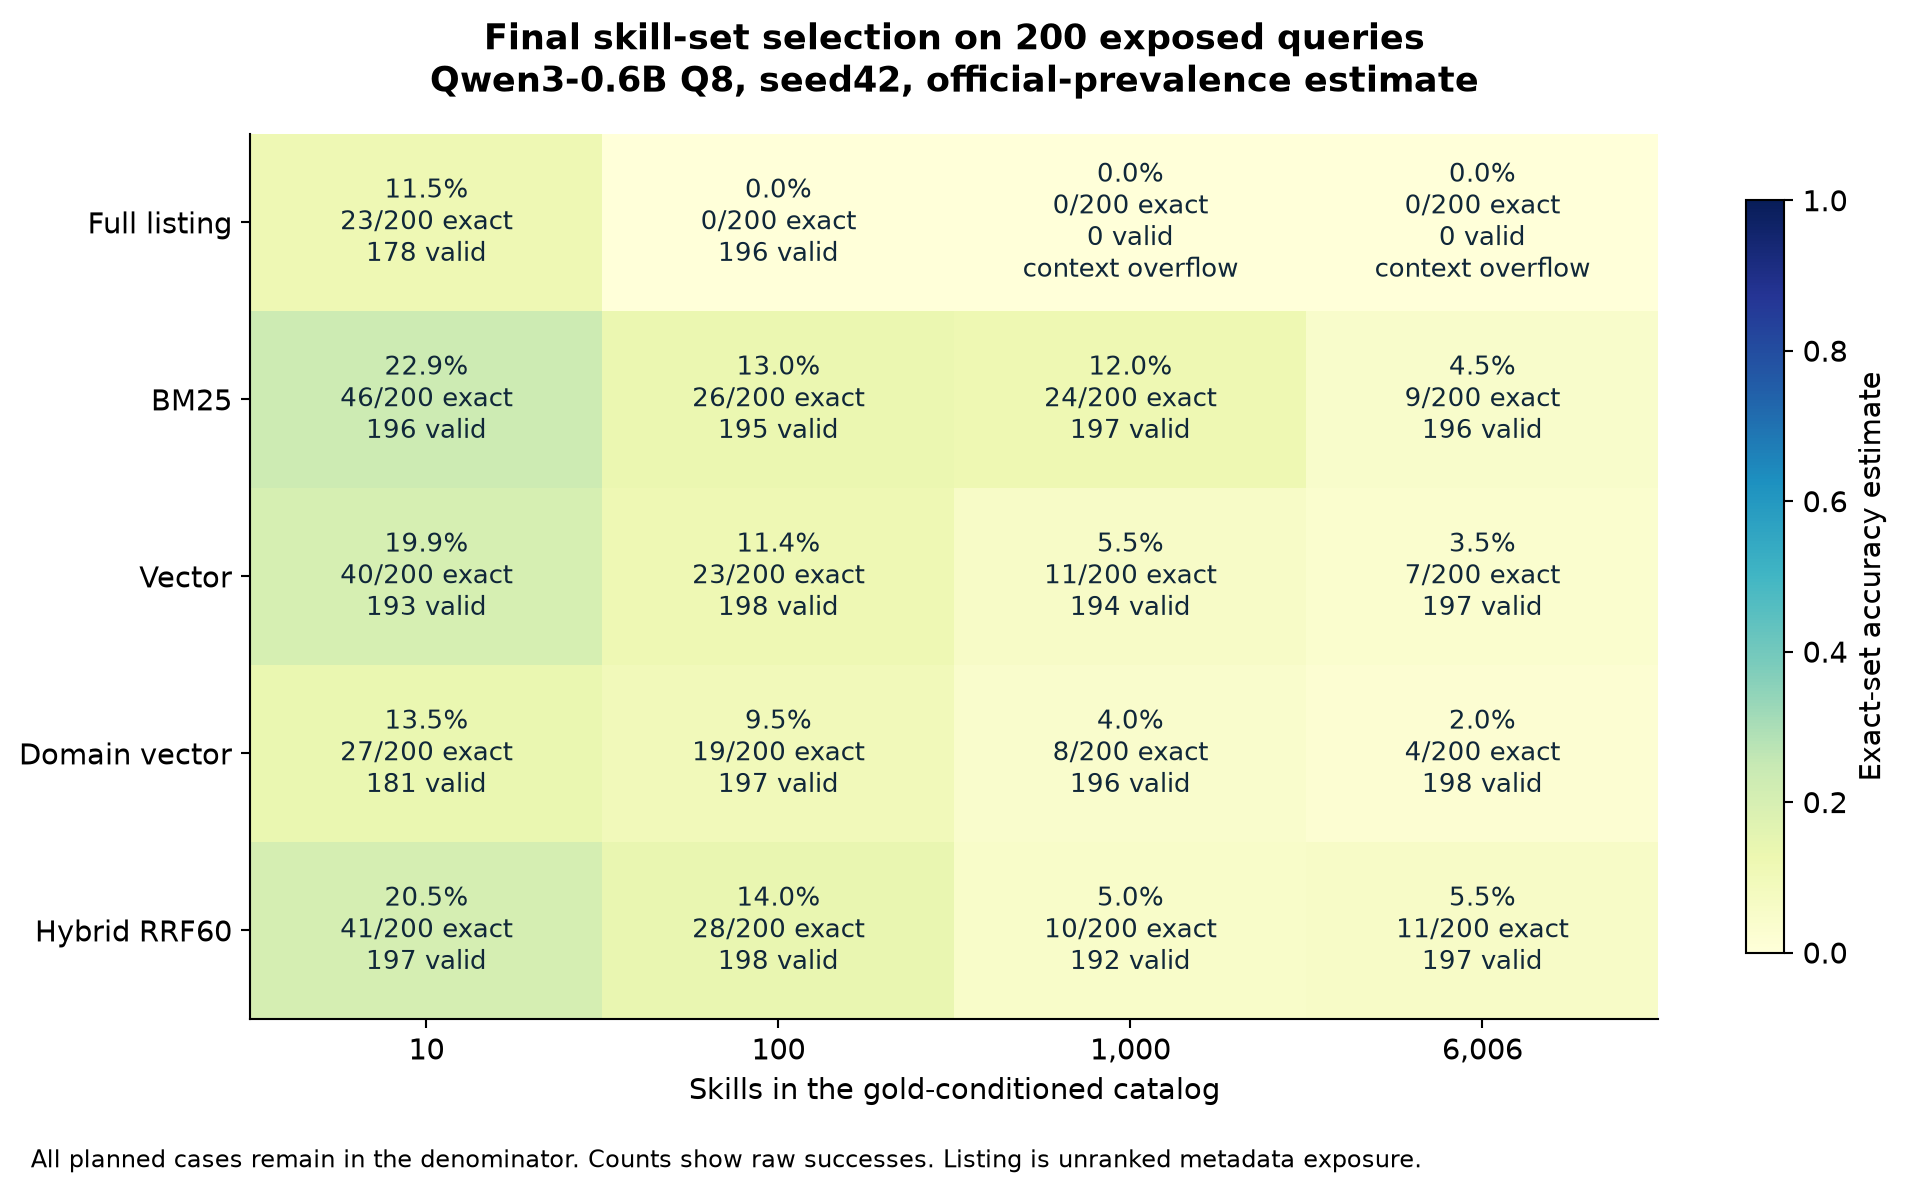
\includegraphics[width=\linewidth]{../experiments/benchmarks/skillret-gap-closure-20261024/report/selection-heatmap.png}\caption{All-planned exact-set agreement. Counts retain 200 queries per cell.}\end{figure}
\section{Analysis and uncertainty}The primary estimate weights strata by official prevalence. Paired query bootstrap resamples within strata using 2,000 fixed-seed replicates. Primary contrasts are hybrid minus BM25 and domain vector minus vector at each size. Report nominal 95\% and family-adjusted percentile intervals. At 6,006, hybrid minus BM25 is +1.02 percentage points with a 95\% interval spanning zero. More context does not guarantee correct selection: at 100 skills, 196 valid listing outputs produced zero exact sets.
\section{Measurement and limitations}Preserve RAM stops, context exclusions, malformed outputs, unknown usage and persistence failures. Early domain timing scored the whole catalog before filtering; corrected timing uses the routed subset and matched implementation cohorts. All public queries were previously exposed. Positive qrels may be incomplete. Generated probes use silver unions without human adjudication. Balanced 24-query model/seed sensitivity remains separate. Two deployments vary architecture/training/quantization, so differences are not purely model-size effects. Ordering, fresh human requests and task execution remain unevaluated.
\section{Conclusion}This bounded local experiment distinguishes candidate coverage, final selection and operational feasibility. It supports reproducible comparison and explicit limits rather than a universal method ranking.
\section*{Contributions and AI assistance}Team aliases are preserved. Contributions await team confirmation. This AI-assisted research draft requires human review; no completed human adjudication is claimed.
\bibliographystyle{plain}\bibliography{references}
\appendix\section{Audit and reproduction}The study contains frozen protocols, exact catalogs, source snapshots, full raw outputs and compact independently scoreable cells. Run aggregate.py, plot.py, compact\_audit.py and make\_report.py. The original 80-cell crosswalk and 30-row closure matrix retain pending human and hosted work. The balanced model/seed and generated-probe tables are in the accompanying report.
\section{Separate hosted diagnostic follow-up}After the immutable local data snapshot, a versioned 24-query balanced exposed panel at 100 skills was run with Qwen3-30B-A3B-Instruct-2507 through SiliconFlow. All 120 method cases were valid. Exact sets were 5/24 for listing, 13/24 for BM25, 7/24 for vector, 4/24 for domain vector and 10/24 for hybrid. These are diagnostic balanced-panel rates, not official-prevalence estimates or a causal local-versus-hosted model comparison. The output wrapper and timing scope differ from the local experiment. All 147 Qwen requests, including canaries and routing, reported charges totaling US\$0.02411946. Two earlier failed provider canaries retain unknown actual costs and US\$0.16 conservative liability holds. The guarded total is US\$0.18411946 across 149 generation attempts. Original hosted cells and human adjudication remain incomplete. Saved raw outputs, cost ledger and descriptive paired uncertainty accompany the separate hosted report; this appendix does not alter the validated local PDF snapshot.
\end{document}
